\label{Section:approach}
In this work, we are trying to explore the trade-offs among  power, performance and quality of exascale simulation applications.  These simulation applications are based on Adaptive Mesh Refinement (AMR) method, which  is a method of dynamically adapting the solution's resolution within certain region of simulation. In 1984, Berger and Oliger proposed using AMR for computing time-dependent solutions to hyperbolic partial differential equations in multiple space dimensions. \cite{berger1984adaptive} Later on, they and Phillip Colella developed local adaptive mesh refinement algorithm for dynamic gridding.\cite{berger1989local} And since then, this AMR approach has been used in solving or simulating a variety engineering problems.\cite{berger1984adaptive,powell1993adaptive,bell1994three} The beauty of AMR is that it only focus computational resources in regions of interest but decrease solution's resolution in regions with less interest. By doing this, it largely increases computational utilization and therefore minimizes memory and storage requirements. It is powerful especially in solving problems with multiple scales. 

AMR algorithm uses a hierarchical grid structure, which typically is composed of rectangular in various sizes. The basic adaptive refinement strategy is to refine on logically rectangular patches. From very beginning, the entire problem domain is covered by level 0 grids. As time step moves on, some rectangular portions of level 0 grid are covered by level 1 grids which refined by refinement factor \textit{R} in each direction. Then, regions of each level 1 grid might be covered by level 2 grids, and so on. \cite{AMRalgorithms} Between each step, there is synchronization operations that insure correct behavior at the coarse-fine interfaces, and regridding operations which permit the refined grids to track complex and /or interesting regions of the flow. Therefore, as the level of refinement increase, the number of grids increase  geometrically. These simulation applications using AMR method, on the one hand will  improve computational utilization, on the other hand , the workload will largely increase as they increase solution resolution. 

At meantime, current HPC applications by default are consuming all computational resource and  typically running for relatively long time and usually under certain power budget as well. In this case, if there is a small but urgent work need to be done. How to schedule it to run? From this point of view, we want to investigate if we can create some power budget and computational resource from the current running task while not affect their performance to run other extra tasks. In order to create this power budget, there are two obvious factors we can change, the simulation resolution, and the CPU power.  

In order to explore the trade-offs, we first evaluated the relationship among AMR refinement resolution, CPU power level and the energy consumption. As shown in the Figure \ref{fig:Energy_consumption_trend}, we execute a simulation application, the execution time will increase as the level of refinement/resolution increases or cap down CPU power. The energy consumption presents the same trend as the execution time. The question here is how to use this characterization to create available power budget. We propose to combine these two factors, adjusting resolution and applying appropriate power capping, to get available power budget.

To further demonstrate this concept, we measure the LMC execution time (will replace it with another application) with different resolution levels on 64 cores, as shown in Figure \ref{fig:LMCruntime}. Obviously, the execution time is decreasing as we degrading the resolution levels. In the meantime, capping down the CPU power will increase the execution time. Therefore, if applying appropriate power capping to it, then each execution can be the same. In the work, since we define the execution time as the performance criteria, by adjusting resolution and applying appropriate power capping, we can keep the performance while having the available power budget, shown as the red shadow area in Figure \ref{fig:Available_power_budget}.
Also, by doing so, the memory pressure release a lot, by XX percentage. Since the AMR workload reduce (decrease level of refinement, will reduce the amount of grids), the I/O usage is release a lot, as well. 
























\textbf{Configuration}
\begin{table}[H]
\begin{center}
\begin{tabular}{|l|l|}
	\hline
	\textbf{Parameter} & \textbf{Value}\\ \hline
    Platform & CAPER cluster\\ 		\hline
    Number of cores & 64 cores\\
	\hline
	Resolution & level 3 2 1\\
    \hline
    Time step & 10\\
    \hline
    Time unit & Second\\
    \hline
    Power measurement & RAPL meter\\
    \hline
    Power cap & RAPL\\
    \hline
\end{tabular}
\end{center}
\caption{Configuration for experiment of getting available power budget through power capping and resolution degradation
}
\label{table:table_tradeoff}
\end{table}



\begin{figure}[H]
	\centering
    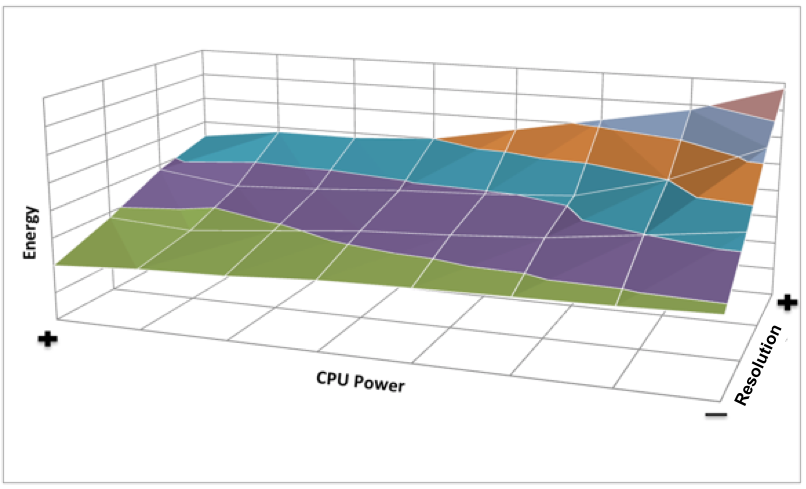
\includegraphics[width=8cm]{figs/Energy_consumption_trend.png}
        \caption{Energy consumption trend for different power caps and refinement levels}
        \label{fig:Energy_consumption_trend}
\end{figure}

\begin{figure}[H]
	\centering
    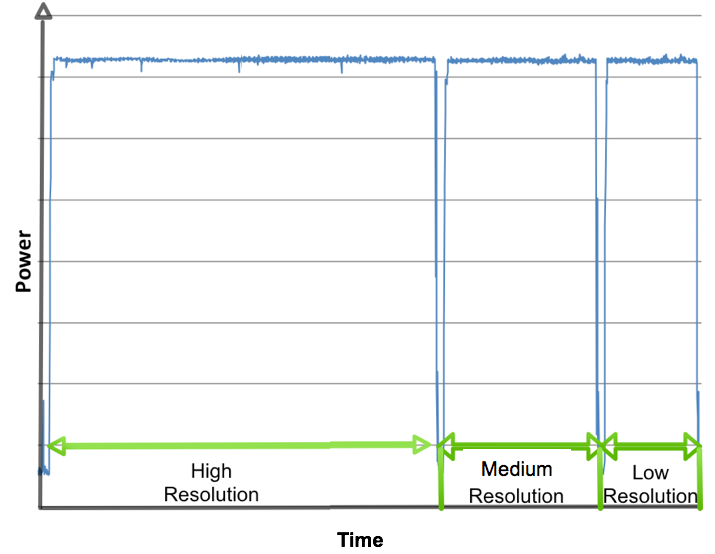
\includegraphics[width=8cm]{figs/LMCruntime.png}
        \caption{LMC power consumption curve with different (qualitative) resolution levels on 64 cores}
        \label{fig:LMCruntime}
\end{figure}


\begin{figure}[H]
	\centering
    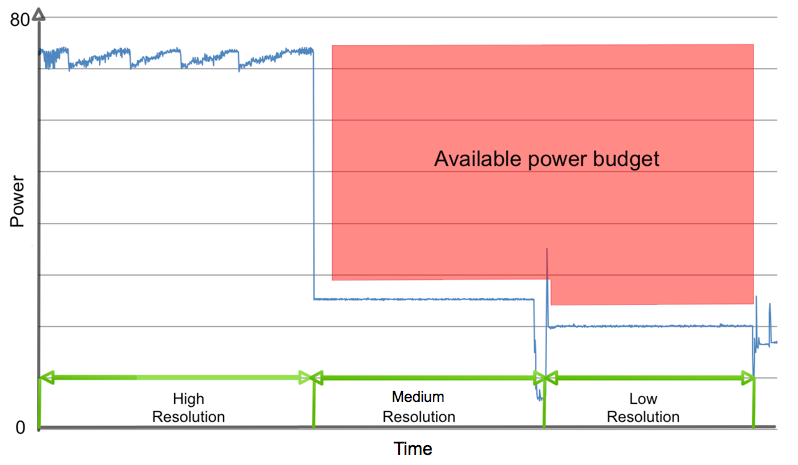
\includegraphics[width=8cm]{figs/Available_power_budget.png}
        \caption{Available power budget from applying resolution degradation and appropriate power capping}
        \label{fig:Available_power_budget}
\end{figure}




















































